% !TeX spellcheck = pl_PL
% -- Rozdział ten może być sprawozdaniem z procesu systematycznego testowania programu. Powinien
% -- zawierać odpowiednio przygotowane dane testowe wraz z formalnym uzasadnieniem ich doboru i
% -- ilości. W dokumentacji umieszczamy wyniki działania programu dla konkretnych danych testowych z
% -- opisem. W tym rozdziale należy umieścić wynik działania programu dla danych wejściowych. Można
% -- tu umieścić np. zrzut ekranu lub wydruk zawartości pliku wynikowego.
\newpage
\part{\huge \textbf{Testowanie i uruchamianie}}
	W naszej grze korzystamy z zasobów przechowywanych w plikach. Są to zarówno pliki sprajtów (\emph{resources}), które są wczytywane i wyświetlane oraz pliki XML, które zawierają informacje na temat konfiguracji gry oraz logikę sceny (\emph{stages}) - w której sekundzie mają się pojawić jacy wrogowie, jak strzelać, w którą stronę się poruszać, co się dzieje gdy zostaną zabici itp. Wszystkie te pliki są niezbędne do prawidłowego działania gry. W przypadku, gdy któregoś brakuje, program o tym informuje oraz odmawia uruchomienia wybranego modułu.
	\section{Config.xml}
		W tym pliku są zawarte informacje o grze, które można dynamicznie zmieniać przez menu \emph{Options}. Format pliku wygląda następująco:
		\begin{lstlisting}[language=xml]
		<Config>
			<Lifes number="6"/>
			<Bombs number="4"/>
			<Controls>
				<Key type="UP" 		key="UPARROW"/>
				<Key type="DOWN" 	key="DOWNARROW"/>
				<Key type="LEFT" 	key="LEFTARROW"/>
				<Key type="RIGHT" 	key="RIGHTARROW"/>
				<Key type="SHOOT" 	key="Z"/>
				<Key type="BOMB" 	key="X"/>
				<Key type="FOCUS" 	key="LSHIFT"/>
			</Controls>
		</Config>
		\end{lstlisting}
		W przypadku nieprawidłowego formatu tego dokumentu, program zwróci komunikat o błędzie i zamknie program. Gra nie może zostać prawidłowo uruchomiona, jeśli program nie zna klawiszy sterujących lub początkowej liczby żyć i bomb.
	\section{Scores.xml}
		W tym pliku znajdują się informacje o zapisanych wynikach z poprzednich rozgrywek: każdy rekord składa się z nicku gracza, wyniku punktowego i daty zapisania. Format pliku wygląda następująco:
		\begin{lstlisting}[language=xml]
			<?xml version="1.0" encoding="UTF-8"?>
			<Scores>
				<Entry nick="Ervelan"  score="1234567" date="2015-05-31"/>
				<Entry nick="Son Mati" score="9876543" date="2015-06-01"/>
				<Entry nick="Trimack"  score="69"      date="2015-06-06"/>
				<Entry nick="Doxus"    score="1313131" date="2015-05-27"/>
			</Scores>
		\end{lstlisting}
		W przypadku nieprawidłowego formatu tego dokumentu, program uruchomi się poprawnie, ale nie będzie możliwe wejście do podmenu \emph{Scores}, ani uruchomienie nowej gry (zostanie zwrócony komunikat o błędzie). Nie można wyświetlić złych wyników, ani uruchomić gry, jeśli zapisanie wyniku będzie niemożliwe.
	\newpage
	\section{Stage.xml}
		W tym pliku znajdują się wszystkie informacje o wyglądzie planszy do gry. Jest to tak naprawdę najważniejszy plik w całej grze, bez którego gameplay jest fundamentalnie niemożliwy. Stage zawiera m.in. takie informacje jak:
		\begin{itemize}
			\item Kto kiedy atakuje?
			\item Jak atakuje?
			\item Jak się porusza? Z jaką prędkością? Z jakim przyspieszeniem?
			\item Jak się poruszają pociski? W którą stronę lecą?
			\item Jak wygląda przeciwnik? Jak wyglądają jego pociski?
			\item Co się stanie, jak zginie?
			\item Czy to już ostatni przeciwnik?
		\end{itemize}
		Podstawowym elementem w tym pliku jest gałąź \textbf{Time}. Mówi ona co ma się stać w której sekundzie (jest to wystarczająca precyzja dla atrakcyjnej rozgrywki), mianowicie jacy wrogowie mają się pojawić wraz z całą ich konfiguracją.\\Plik ten jest wczytywany po uruchomieniu nowej gry, analizowany, a na jego podstawie są tworzone elementy na planszy. Jeżeli plik nie istnieje, jego format jest nieprawidłowy, lub dane są nieczytelne, program wyrzuca wyjątek, informuje użytkownika o zaistniałym błędzie i zamyka grę, wracają do ekranu powitalnego.
		\newpage
		\subsection{Testowanie planszy}
		Format tego pliku oraz sposób jego parsowania przeszedł ogromną liczbę testów, aż w końcu osiągnął kształt, jaki prezentują następujące dane wejściowe.
		\subsubsection{Pojedynczy wróg}
		\begin{lstlisting}[language=xml]
			<Time sec="1" type="normal">
				<Enemy number="1" distance="96" start="-32" image="YukkuriReimu" life="100" speed="450" length="700">
					<Bonus type="Power" number="5" value="0.1"></Bonus>
					<Trajectory type="Line" startPoint.x="LEFT" startPoint.y="ONE_THIRDS" a="0"></Trajectory>
					<Pattern type="Line" par1="-75" bulletNumber="5" number="10" interval="0.1">
						<Bullet image="BulletBlueCircle" speed="96" width="32" height="32" hitboxSize="HALF"></Bullet>
					</Pattern>
				</Enemy>
			</Time>
		\end{lstlisting}
		W powyższym przykładzie zaprezentowano atak pojedynczego wroga. Dokładnie mówi on:
		\begin{enumerate}
			\item W pierwszej sekundzie pojawia się jeden zestaw wrogów składający się z jednego wroga.
			\item Wróg ten posiada sprajt YukkuriReimu, 100 punktów życia i porusza się z prędkością 450 punktów na sekundę.
			\item Po przebyciu dystansu 700 punktów zostaje on usunięty z planszy.
			\begin{enumerate}
				\item Jeśli zostanie zabity, wyleci z niego 5 bonusów typu Power o wartości 0.1
				\item Ów wróg porusza się po torze liniowym, z punktem początkowy po lewej stronie ekranu oraz jednej trzeciej ekranu w pionie.
				\item Kąt linii względem układu współrzędnych jest równy 0 stopni - wróg porusza się więc z lewej strony ekranu ku prawej.
				\item Wróg posiada jeden typ wzoru (\emph{patternu}):
				\begin{enumerate}
					\item Jego pociski poruszają się po torze liniowym, pod kątem -75 stopni, czyli prawie idealnie ku dołowi ekranu.
					\item Wróg atakuje 10 takimi wzorami, z czego każdy składa się z 5 pocisków
					\item Pociski są wystrzeliwane w odstępie 0.1 sekundy
					\begin{enumerate}
						\item Kształt pocisków to sparjt BulletBlueCircle o wymiarach 32 x 32.
						\item Pociski poruszają się z prędkością 96 punktów na sekundę
						\item Średnica hitboxa pocisków jest równa połowie ich boku
					\end{enumerate}
				\end{enumerate}
			\end{enumerate}
		\end{enumerate}
		Wszystkie wartości, jakie nie zostały zdefiniowane w tym przykładzie, przyjmują wartości domyślne, np. przyspieszenie wszystkich obiektów jest równe zeru.\\
		Efekt jest następujący:
		\begin{center}
			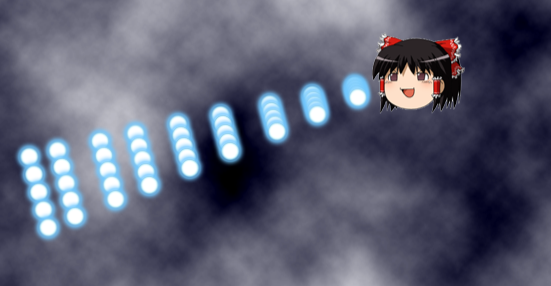
\includegraphics[width=0.6\textwidth]{./images/test1}
		\end{center}
		
		
		\newpage
		\subsubsection{Atak krzyżowy}
		W poniższym przykładzie zaprezentowano "atak krzyżowy" - dwóch przeciwników atakuje z lewej i prawej strony planszy, bombardując gracza pociskami.
		\begin{lstlisting}[language=xml]
		<Time sec="4" type="normal">
			<Enemy number="3" distance="96" start="-32" image="YukkuriReimu" life="150" speed="450" length="700">
				<Bonus type="Power" number="5" value="0.1"></Bonus>
				<Trajectory type="Line" startPoint.x="LEFT" startPoint.y="ONE_THIRDS" a="0"></Trajectory>
				<Pattern type="Line" par1="-75" bulletNumber="5" number="15" interval="0.1">
					<Bullet image="BulletBlueCircle" speed="96" acc="50.0" width="32" height="32" hitboxSize="HALF"></Bullet>
				</Pattern>
			</Enemy>
			<Enemy number="3" distance="96" start="-32" image="YukkuriReimu" life="575" speed="-450" length="700">
				<Bonus type="Score" number="5" value="1000"></Bonus>
				<Trajectory type="Line" startPoint.x="RIGHT" startPoint.y="ONE_THIRDS" a="0"></Trajectory>
				<Pattern type="Line" par1="-105" bulletNumber="5" number="15" interval="0.1">
					<Bullet image="BulletRedCircle" speed="96" acc="50.0" width="32" height="32" hitboxSize="HALF"></Bullet>
				</Pattern>
			</Enemy>
		</Time>
		\end{lstlisting}
	 	Dokładnie mówi on:
		\begin{enumerate}
			\item W czwartej sekundzie mają się pojawić dwa zestawy normalnych wrogów.
			\item W obu zestawach występuje po 3 wrogów - między nimi jest 96 punktów dystansu zgodnie z trajektorią po jakiej się poruszają. Wszyscy znajdują się o 32 punkty dystansu z tyłu od punktu początkowego.
			\item Wrogowie z pierwszego zestawu mają 150 życia i prędkość 450, z drugiego 575 życia i -450 szybkości (poruszają się zgodnie z przeciwnym kierunkiem). Wszyscy znikają po przebyciu 700 punktów dystansu.
			\item Wszyscy poruszają się po tej samej linii prostej, ale każdy zestaw w przeciwnym kierunku.
			\item Kąty wzorów są dostosowane tak, by wyglądały estetycznie: -75 oraz -105 sprawiają, że pociski poruszające się również po linii się krzyżują.
			\item Pociski pierwszego zestawu są niebieskie, a drugiego czerwone. Pozostałe parametry są jednakowe.
			\item Pociski posiadają przyspieszenie równe 50 - oznacza to, że co sekundę ich szybkość zwiększa się o 50 punktów na sekundę.
		\end{enumerate}
		\begin{center}
			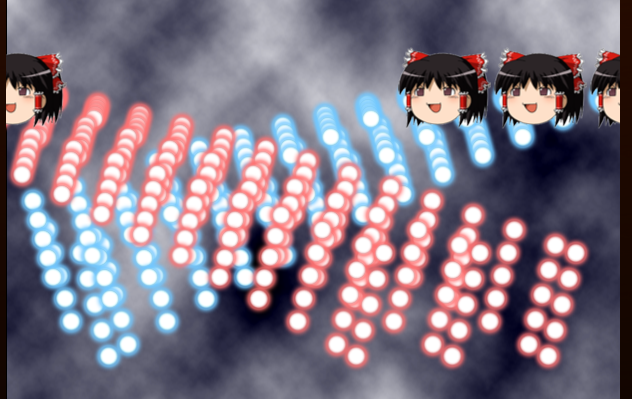
\includegraphics[width=0.51\textwidth]{./images/test2}
		\end{center}
		
		\newpage
		\subsubsection{Ruch po linii łamanej}
		Ten przykład pokazuje działanie klasy TrajectoryManyPoints - w niej obiekt porusza się od punktu do punktu.
		\begin{lstlisting}[language=xml]
		<Time sec="9" type="normal">
			<Enemy number="7" distance="32" start="32" image="YukkuriCirno" life="100" speed="200" length="800">
				<Bonus type="Power" number="3" value="0.1"></Bonus>
				<Trajectory type="Polygon">
					<Point x="LEFT"  y="TWO_THIRDS"></Point>
					<Point x="LEFT"  y="ONE_THIRDS"></Point>
					<Point x="RIGHT" y="ONE_THIRDS"></Point>
					<Point x="RIGHT" y="TWO_THIRDS"></Point>
					<Point x="LEFT"  y="TWO_THIRDS"></Point>
				</Trajectory>
				<Pattern type="Line" par1="-75" bulletNumber="5" number="20" interval="0.3">
					<Bullet image="BulletYellowCircle" speed="96" width="32" height="32" hitboxSize="HALF"></Bullet>
				</Pattern>
			</Enemy>
		</Time>
		\end{lstlisting}
		Konieczne jest zdefiniowanie kilku punktów, zagnieżdżonych w gałęzi Trajectory. Kod mówi, że:
		\begin{enumerate}
			\item W 9 sekundzie pojawia się 7 przeciwników, o kształcie YukkuriCirno, oddalonych od siebie o 32 punkty porusza się z prędkością 100 punktów na sekundę po wieloboku zdefiniowanym punktami w gałęziach \textbf{Point}.
			\item Każdy z nich wyrzuca z siebie 3 bonusy typu Power oraz atakuje pociskami poruszającymi się po linii.
			\item Odstęp czasowy między kolejnymi strzałami to 0.3 sekundy
		\end{enumerate}
		Efekt jest oczekiwany:
		\begin{center}
			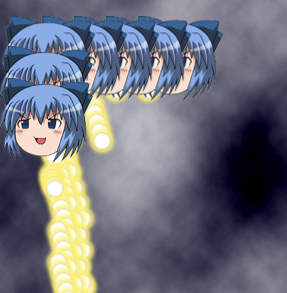
\includegraphics[width=0.50\textwidth]{./images/test3}
		\end{center}
		
		\newpage
		\subsubsection{Bardziej zaawansowany przykład}
		\begin{lstlisting}[language=xml]
			<Time sec="1" type="normal">
				<Enemy number="1" start="0" image="YukkuriKoishi" life="4000" speed="0" length="500">
					<Bonus type="Score" number="10" value="0.1"></Bonus>
					<Trajectory type="None" center.x="HALF" center.y="HALF" a="0"></Trajectory>
					<Pattern type="Bezier" bulletNumber="1" number="30" interval="0.20">
						<Bullet image="BulletRedCircle" speed="200" width="40" height="40" hitboxSize="FULL"></Bullet>
						<Point x="307"  y="253"></Point>
						<Point x="568"  y="111"></Point>
						<Point x="692"  y="467"></Point>
						<Point x="337"  y="723"></Point>
					</Pattern>
					<Pattern type="Bezier" bulletNumber="1" number="30" interval="0.20">
						<Bullet image="BulletRedCircle" speed="200" width="40" height="40" hitboxSize="FULL"></Bullet>
						<Point x="307"  y="253"></Point>
						<Point x="146"  y="111"></Point>
						<Point x="22"   y="467"></Point>
						<Point x="337"  y="723"></Point>
					</Pattern>
					<Pattern type="Line" par1="-30" bulletNumber="5" number="5" interval="1.0">
						<Bullet image="BulletHeart" speed="96" acc="50.0" width="32" height="32" hitboxSize="HALF">
							<Affine scale="1.8" rotate="4.0"></Affine>
						</Bullet>
					</Pattern>
					<Pattern type="Line" par1="-60" bulletNumber="5" number="5" interval="1.0">
						<Bullet image="BulletHeart" speed="96" acc="50.0" width="32" height="32" hitboxSize="HALF">
							<Affine scale="1.8" rotate="4.0"></Affine>
						</Bullet>
					</Pattern>
					<Pattern type="Line" par1="-90" bulletNumber="5" number="5" interval="1.0">
						<Bullet image="BulletHeart" speed="96" acc="50.0" width="32" height="32" hitboxSize="HALF">
							<Affine scale="1.8" rotate="4.0"></Affine>
						</Bullet>
					</Pattern>
					<Pattern type="Line" par1="-120" bulletNumber="5" number="5" interval="1.0">
						<Bullet image="BulletHeart" speed="96" acc="50.0" width="32" height="32" hitboxSize="HALF">
							<Affine scale="1.8" rotate="4.0"></Affine>
						</Bullet>
					</Pattern>
					<Pattern type="Line" par1="-150" bulletNumber="5" number="5" interval="1.0">
						<Bullet image="BulletHeart" speed="96" acc="50.0" width="32" height="32" hitboxSize="HALF">
							<Affine scale="1.8" rotate="4.0"></Affine>
						</Bullet>
					</Pattern>
				</Enemy>
			</Time>
		\end{lstlisting}
		\newpage
		\textbf{Najistotniejsze rzeczy w powyższym kodzie}:
		\begin{enumerate}
			\item Przeciwnik jest jeden i posiada 400 punktów życia - umrze dopiero po dłuższym czasie.
			\item Typ jego trajektorii to \textit{None}, innymi słowy, może tylko stać w miejscu, wyznaczonym jako środek planszy.
			\item Przeciwnik posiada łącznie 7 różnych typów wzorów:
			\begin{itemize}
				\item Pierwsze dwa zbudowane są na krzywych Beziera wyznaczonych przez gałęzie \textbf{Point} (pierwszy jest początkowy, a ostatni końcowy). Pociski na obu krzywych poruszają się jednakowo i mają ten sam kształt.
				\item Parametry punktów zostały dobrane tak, żeby każda z krzywych tworzyła połowę serca.
				\item Pozostałe 5 wzorów wykorzystuje pociski w kształcie serc, które poruszają się po liniach z jednakową szybkością i przyspieszeniem.
				\item Każdy ze wzorów jest "oddalony" o kolejne 30 stopni.
				\item Te wzory posiadają również gałęzie \textbf{Affine} - oznaczają one, że ich pociski w czasie pojedynczej sekundy zwiększają swój rozmiar 1.8-krotnie oraz obracają się wokół własnej osi o 4 stopnie.
			\end{itemize}
			\item Te wzory mają razem tworzyć estetycznie wyglądającą całość, co widać poniżej.
		\end{enumerate}
		\begin{center}
			
\includegraphics[width=0.60\textwidth]{./images/test4}
		\end{center}
		
		
		
		
		
		